\documentclass{article}

% Package necessari
\usepackage[a4paper]{geometry}
\usepackage[utf8]{inputenc}
\usepackage[italian]{babel}
\usepackage[T1]{fontenc}
\usepackage[font={small,sl}]{caption}
\usepackage[font={small,sl}]{subcaption}
\usepackage{graphicx}
\usepackage[usenames, table, dvipsnames]{xcolor}
\usepackage{hyperref}
\usepackage[most]{tcolorbox}
\usepackage[section]{placeins}
\usepackage{soulutf8}
\usepackage{listings}
% \usepackage{hhline}

% Titolo del documento
\title{\small Relazione progetto Sistemi Operativi Avanzati \\
\Huge \textbf{Multi-flow Device File}}

% Autore del documento
\author{Simone Tiberi (M. 0299908)\\%
(email: \texttt{\href{mailto:simone.tiberi.98@gmail.com}{simone.tiberi.98@gmail.com}})}

% Data del documento
\date{\today}

% Impostazione delle lunghezze di alcuni elementi del documento
\setlength{\parskip}{1em}
\setlength{\parindent}{0em}

% Impostazioni del package hyperref
\hypersetup{
        colorlinks=true,
        linktocpage=true,
        linkcolor=blue,
        urlcolor=blue,
        pdftitle={Relazione progetto SOA},
        pdfauthor={Simone Tiberi},
}

\lstset{
	language=C,
	frame=shadowbox,
	rulesepcolor=\color{gray!50},
	basicstyle=\ttfamily\small,
	keywordstyle=\color{purple}\bfseries\small,
	stringstyle=\color{ForestGreen}\small,
	commentstyle=\color{blue}\small,
	numbers=left,
	numberstyle=\small\color{gray},
	numbersep=5pt,
	tabsize=2,
	showtabs=false,
	showspaces=false,
	showstringspaces=false,
	escapechar=|,
	captionpos=b,
	breaklines=true,
	keepspaces=true
}

\renewcommand{\lstlistingname}{Listato}
\graphicspath{ {./figs/} }

\newtcolorbox{nb}[1]{
        colframe = blue!25,
        colback  = blue!10,
        coltitle = blue!20!black,
        title    = #1,
        breakable,
        enhanced,
}

% Tabelle
\renewcommand{\arraystretch}{1.5}
\setlength{\arrayrulewidth}{0.1em}

\begin{document}
\maketitle

\section*{Specifica del progetto (traduzione)}
La specifica richiede l'implementazione di un device driver per Linux per la gestione di flussi di dati a due livelli di priorità. Attraverso una sessione aperta verso un dispositivo, un thread può leggere/scrivere dati in modo tale che:
\begin{itemize}
        \item la consegna dei dati segua una politica \textbf{FIFO} (\textbf{F}irst-\textbf{I}n-\textbf{F}irst-\textbf{O}ut),
        \item non appena letti i dati \textbf{scompaiano} dal flusso,
        \item la scrittura sul flusso ad alta priorità sia \textbf{sincrona},
        \item la scrittura sul flusso a bassa priorità sia \textbf{asincrona}, basata su deferred work, \ul{mantenendo comunque la sincronia nella notifica dell'esito dell'operazione} (in conformità all'interfaccia della \texttt{write}),
        \item la scrittura sia sempre eseguita in modo sincrono,
        \item il driver supporti al più \textbf{128} devices associati al corrispettivo minor number.
\end{itemize}

Il device driver deve implementare il supporto all'operazione \texttt{ioctl} al fine di gestire le sessioni di I/O e permettere:
\begin{itemize}
        \item di impostare il livello di priorità (\texttt{HIGH} or \texttt{LOW}) per le operazioni,
        \item di scegliere se effettuare letture e/o scritture in modo bloccante o meno,
        \item di impostare un timeout per regolare il risveglio in caso di richieste bloccanti
\end{itemize}

Inoltre è richiesto di implementare un meccanismo per abilitare o disabilitare i dispositivi in termini di minor numbers, basato sui parametri del modulo. Nel caso in cui un dispositivo sia disabilitato, ogni tentativo di apertura di nuova sessione deve fallire, ma devono comunque continuare ad essere gestite quelle aperte in precedenza.

Altri parametri addizionali esposti tramite VFS devono fornire un'immagine dello stato corrente dei device in termini di:
\begin{itemize}
        \item stato corrente (\texttt{ENABLED} o \texttt{DISABLED}),
        \item numero di byte correntemente presenti nei due flussi,
        \item numero di thread correntemente in attesa nei due flussi
\end{itemize}

\section*{Struttura del repository}
La realizzazione della specifica è stata organizzata all'interno del repository nelle seguenti cartelle:
\begin{itemize}
        \item nella radice è presente uno script \texttt{bash} per la creazione di nodi di I/O pilotabili con il driver sviluppato,
        \item in \texttt{KERNEL\_MODULE/} è contenuto il codice effettivo del driver,
        \item in \texttt{USER\_LIB/} è contenuta una libreria utente per facilitare l'interfacciamento utente con i nodi di I/O associati al driver sviluppato,
        \item in \texttt{SAMPLES/} sono presenti una semplice demo e un file contenente diversi test cases
\end{itemize}

\section*{Driver per la gestione dei dispositivi multi-flusso}
Per gestire i dati associati al device $i$-esimo (con $0\leq i\leq127$), la scelta implementativa è ricaduta sull'utilizzo di un buffer circolare, così come mostrato in figura \ref{fig:buffer}. Per via della politica di gestione \texttt{FIFO} richiesta dalla specifica, è stato sufficiente mantenere l'indice di inizio della zona \textit{valida} e la sua taglia. La \textit{valid zone} rappresenta l'area, non necessariamente contigua per via della circolarità del buffer, in cui sono presenti i dati scritti, ma non ancora letti.

\begin{figure}[htbp]
        \centering
        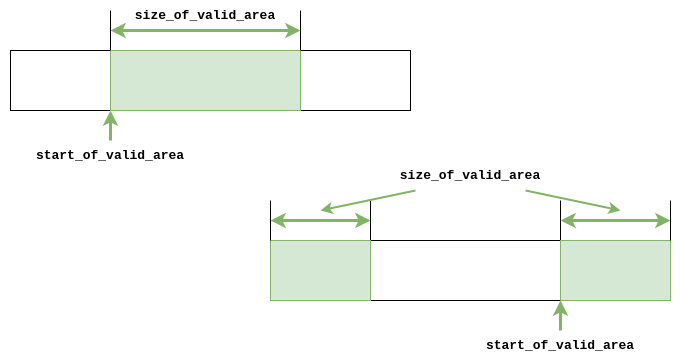
\includegraphics[width=.8\textwidth]{buffer}
        \caption{Rappresentazione in memoria dei dati associati al dispositivo sotto forma di buffer circolare}
        \label{fig:buffer}
\end{figure}

Istante per istante, è possibile ricavare l'indice di successiva scrittura computandolo come segue:
\[
        \mathtt{next\_write} = (\mathtt{start\_of\_valid\_area} + \mathtt{size\_of\_valid\_area})\ \%\ \mathtt{BUFSIZE}
\]
dove per \texttt{BUFSIZE} è stato scelto \texttt{PAGE\_SIZE}, ovvero 4096 B.

Logicamente ciascuno dei 128 dispositivi supportati dal device driver è stato rappresentato tramite la struttura dati \texttt{device\_state} la quale molto semplicemente contiene al suo interno:
\begin{itemize}
        \item il vettore di due elementi strutturati secondo la regola \texttt{data\_flow} di seguito analizzata,
        \item il puntatore ad una work queue necessaria per la gestione delle scritture \textit{deferred} nel caso \texttt{LOW\_PRIO}.
\end{itemize}

La struttura dati \texttt{data\_flow} è la principale in tutta l'architettura e raccoglie al suo interno i campi necessari alla gestione del singolo flusso di dati associato al dispositivo, quali:
\begin{itemize}
        \item il buffer in/da cui scrivere/leggere i dati,
        \item la posizione dell'inizio dell'area valida all'interno del buffer,
        \item la taglia dell'area valida all'interno del buffer,
        \item il livello di priorità associato al flusso (\texttt{HIGH\_PRIO} oppure \texttt{LOW\_PRIO}),
        \item il \texttt{mutex} per sincronizzare le operazioni ed evitare, ad esempio, che i metadati vengano aggiornati per effetto di una scrittura ed una lettura contemporaneamente,
        \item la wait queue dove accodare le richieste bloccanti nel caso in cui non vi siano dati disponibili in lettura oppure spazio utilizzabile in scrittura,
        \item il numero di bytes \textit{pendenti}, ovvero per i quali è presente una richiesta di scrittura deferred già accettata dal driver, non ancora soddisfatta,
        \item il numero di thread pendenti in attesa vi siano dati disponibili oppure spazio utilizzabile.
\end{itemize}

\end{document}
